\documentclass[10pt]{beamer}
\usetheme{metropolis}

% ── Packages ──
\usepackage{amsmath,amssymb,amsthm}
\usepackage{tikz}
\usetikzlibrary{positioning,arrows.meta,fit,calc,matrix}
\usepackage{graphicx}
\usepackage{array}
\usepackage{xcolor,colortbl}

% ── Theorem environments ──
\theoremstyle{definition}
\newtheorem{defi}{Definition}[section]
\newtheorem{prop}{Proposition}[section]
\newtheorem{thm}{Theorem}[section]
\newtheorem{cor}{Corollary}[section]

% ── Emoji definitions ──
\newcommand{\bean}{
\includegraphics[scale=0.07]{Pictures/bean.png}}
\newcommand{\leaf}{
\includegraphics[scale=0.08]{Pictures/leaf.png}}
\newcommand{\lemon}{
\includegraphics[scale=0.08]{Pictures/lemon.png}}
\newcommand{\cow}{
\includegraphics[scale=0.08]{Pictures/cow.png}}
\newcommand{\bento}{
\includegraphics[scale=0.08]{Pictures/bento.png}}
\newcommand{\milk}{
\includegraphics[scale=0.08]{Pictures/milk.png}}
\newcommand{\coffee}{
\includegraphics[scale=0.08]{Pictures/coffee.png}}
\newcommand{\tea}{
\includegraphics[scale=0.08]{Pictures/tea.png}}

% ── Highlighting ──
\newcommand{\x}[1]{\alert{\textbf{#1}}}

\title{Lecture 4: Linear Independence and Dimension}
\subtitle{Proving Rank is Well-Defined}
\date{}

\begin{document}
\maketitle

% ═══════════════════════════════════════
% §1 MOTIVATION
% ═══════════════════════════════════════
\section{Motivation: Is Rank Well-Defined?}

\begin{frame}{Recall: Rank from Cross-Filling}
In Lecture 3, we defined:

$$\text{rank}(A) = \text{number of rank-one pieces from cross-filling}$$

\vfill
\x{Problem}: Cross-filling allows \x{different pivot choices}.

\vfill
For
$$A = \begin{pmatrix} 2 & 4 & 6 \\ 1 & 2 & 3 \\ 3 & 6 & 9 \end{pmatrix}$$

we could pick pivot at $(1,1)$, or $(2,2)$, or $(3,3)$.

\vfill
\x{Question}: Do all choices give the \x{same number} of pieces?
\end{frame}

\begin{frame}{Today's Goal}
\x{Prove that rank is well-defined} by showing:

$$\boxed{\text{rank}(A) = \text{dimension of column space}}$$

\vfill
\textbf{Strategy}:
\begin{enumerate}
\item Introduce \x{linear independence} and \x{basis}
\item Prove all bases have the \x{same size} (using trace)
\item Show cross-filling produces a \x{basis} for column space
\item Conclude: rank = dimension (well-defined!)
\end{enumerate}
\end{frame}

% ═══════════════════════════════════════
% §2 LINEAR INDEPENDENCE
% ═══════════════════════════════════════
\section{Linear Independence}

\begin{frame}{Linear Independence — Definition}
\begin{defi}[Linear Independence]
Vectors $v_1, v_2, \ldots, v_k$ are \x{linearly independent} if:

$$c_1 v_1 + c_2 v_2 + \cdots + c_k v_k = 0 \quad \Rightarrow \quad c_1 = c_2 = \cdots = c_k = 0$$
\end{defi}

\vfill
In other words: The \x{only} way to make zero is the \x{trivial combination}.
\end{frame}

\begin{frame}{Concrete Example: Coffee Shop Recipe Vectors}
Shinchan's coffee shop has 3 recipe vectors (columns = ingredients):

\vfill
\begin{center}
\begin{tabular}{c|ccc}
& \coffee & \tea & \milk \\
\hline
\bean & 2 & 1 & 0 \\
\leaf & 1 & 2 & 0 \\
\lemon & 0 & 1 & 0 \\
\cow & 1 & 0 & 1
\end{tabular}
\end{center}

\vfill
These are recipe vectors $v_1 = \begin{pmatrix} 2 \\ 1 \\ 0 \\ 1 \end{pmatrix}$, $v_2 = \begin{pmatrix} 1 \\ 2 \\ 1 \\ 0 \end{pmatrix}$, $v_3 = \begin{pmatrix} 0 \\ 0 \\ 0 \\ 1 \end{pmatrix}$

\vfill
\x{Question}: Are these linearly independent?
\end{frame}

\begin{frame}{Testing Independence: Can We Make Zero Recipe?}
We want to test if $c_1 v_1 + c_2 v_2 + c_3 v_3 = 0$ forces $c_1 = c_2 = c_3 = 0$.

\vfill
Think about it physically: Can we combine recipes to get \x{zero of all ingredients}?

$$c_1 \cdot \coffee + c_2 \cdot \tea + c_3 \cdot \milk = \text{nothing}$$

\vfill
\begin{center}
\begin{tabular}{c|c}
Ingredient & Amount \\
\hline
\bean & $2c_1 + 1c_2 + 0c_3 = 0$ \\
\leaf & $1c_1 + 2c_2 + 0c_3 = 0$ \\
\lemon & $0c_1 + 1c_2 + 0c_3 = 0$ \\
\cow & $1c_1 + 0c_2 + 1c_3 = 0$
\end{tabular}
\end{center}
\end{frame}

\begin{frame}{Solution: Backward Substitution}
From the equations:
\begin{align*}
2c_1 + c_2 &= 0 \\
c_1 + 2c_2 &= 0 \\
c_2 &= 0 \\
c_1 + c_3 &= 0
\end{align*}

\vfill
From equation 3: $c_2 = 0$

Substitute into equation 1: $2c_1 = 0 \Rightarrow c_1 = 0$

Substitute into equation 4: $c_3 = 0$

\vfill
\x{Conclusion}: The \x{only} solution is $c_1 = c_2 = c_3 = 0$.

The vectors are \x{linearly independent}!
\end{frame}

\begin{frame}{Key Insight: Independence = No Redundancy}
\x{Linear independence} means:
\begin{itemize}
\item No recipe can be written as a combination of others
\item Each recipe contributes something \x{new}
\item \x{No wasted vectors} in the list
\end{itemize}

\vfill
\x{Linear dependence} would mean:
\begin{itemize}
\item Some recipe is redundant (can be made from others)
\item For example: If \milk = 0.5\coffee + 0.5\tea, then $v_3$ is redundant
\end{itemize}
\end{frame}

% ═══════════════════════════════════════
% §3 LEFT CANCELLATION PROPERTY
% ═══════════════════════════════════════
\section{Left Cancellation Property}

\begin{frame}{Change of Perspective}
\textbf{What we've learned so far:}
\begin{itemize}
\item \x{What} linear independence means (physically: no redundant recipes)
\item \x{How} to test it (check if $c_1v_1 + \cdots + c_k v_k = 0 \Rightarrow$ all $c_i = 0$)
\end{itemize}

\vfill
\begin{alertblock}{From This Point Forward}
We \x{forget about coffee shop recipes} and work with \x{pure matrix algebra}:
\begin{itemize}
\item \textbf{Vectors} $v_1, \ldots, v_k$ become \textbf{matrix columns} $U = \begin{pmatrix} | & & | \\ v_1 & \cdots & v_k \\ | & & | \end{pmatrix}$
\item \textbf{Linear independence} becomes a \textbf{cancellation property}
\end{itemize}
\end{alertblock}

This simplifies our work: we only track \x{matrix operations}, not physical meanings.
\end{frame}

\begin{frame}{Matrix Form of Linear Independence}
Collect vectors $v_1, \ldots, v_k$ as columns of matrix $U$:

$$U = \begin{pmatrix} | & | & & | \\ v_1 & v_2 & \cdots & v_k \\ | & | & & | \end{pmatrix}$$

\vfill
\x{Linear independence} says:
$$U \begin{pmatrix} c_1 \\ c_2 \\ \vdots \\ c_k \end{pmatrix} = 0 \quad \Rightarrow \quad \begin{pmatrix} c_1 \\ c_2 \\ \vdots \\ c_k \end{pmatrix} = 0$$

In other words: $Uc = 0 \Rightarrow c = 0$
\end{frame}

\begin{frame}{Left Cancellation Property}
\begin{prop}[Left Cancellation]
If $U$ has linearly independent columns, then:
$$UP = UQ \quad \Rightarrow \quad P = Q$$
\end{prop}

\vfill
\textbf{Proof}: If $UP = UQ$, then:
$$UP - UQ = 0$$
$$U(P - Q) = 0$$

Since $U$ has linearly independent columns, $U(P-Q) = 0 \Rightarrow P - Q = 0$.

Therefore $P = Q$. $\square$
\end{frame}

\begin{frame}{Why This Matters: Unique Representations}
Left cancellation means \x{unique representation}:

\vfill
If $v_1, \ldots, v_k$ are linearly independent and we write:
$$w = c_1 v_1 + \cdots + c_k v_k$$

then the coefficients $c_1, \ldots, c_k$ are \x{unique}.

\vfill
\x{Proof}: If also $w = d_1 v_1 + \cdots + d_k v_k$, then:
$$U \begin{pmatrix} c_1 \\ \vdots \\ c_k \end{pmatrix} = U \begin{pmatrix} d_1 \\ \vdots \\ d_k \end{pmatrix}$$

By left cancellation: $c_i = d_i$ for all $i$. $\square$
\end{frame}

% ═══════════════════════════════════════
% §4 TRACE AND DIMENSION
% ═══════════════════════════════════════
\section{Trace and Dimension}

\begin{frame}{The Dimension Question}
\begin{defi}[Basis]
A \x{basis} is a list of vectors that is:
\begin{itemize}
\item \x{Linearly independent}
\item \x{Spans} the space (every vector can be written as a linear combination)
\end{itemize}
\end{defi}

\vfill
\x{Question}: If a space has two different bases, do they have the \x{same number} of vectors?

\vfill
\begin{itemize}
\item Basis 1: $e_1, e_2, \ldots, e_n$
\item Basis 2: $w_1, w_2, \ldots, w_m$
\end{itemize}

Is $n = m$?
\end{frame}

\begin{frame}{The Tool: Trace of a Matrix}
\begin{defi}[Trace]
The \x{trace} of a square matrix $A$ is the sum of its diagonal entries:
$$\text{tr}(A) = a_{11} + a_{22} + \cdots + a_{nn}$$
\end{defi}

\vfill
\x{Example}:
$$\text{tr}\begin{pmatrix} 1 & 2 & 3 \\ 4 & 5 & 6 \\ 7 & 8 & 9 \end{pmatrix} = 1 + 5 + 9 = 15$$

\vfill
Key property we need: $\text{tr}(AB) = \text{tr}(BA)$ (even if $A$ and $B$ are \x{not square}!)
\end{frame}

\begin{frame}[fragile]{Visual Proof: $\text{tr}(AB) = \text{tr}(BA)$ — First Diagonal Entry}
Consider $2 \times 3$ matrix $A$ and $3 \times 2$ matrix $B$:

\vfill
\begin{center}
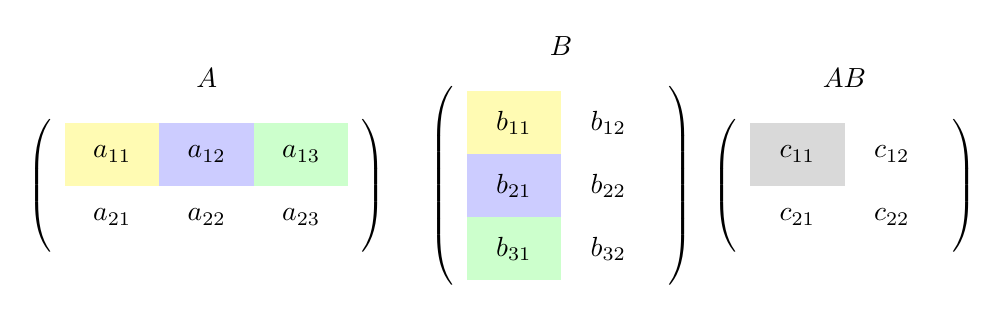
\begin{tikzpicture}[scale=0.9]
% Matrix A
\matrix (A) at (0,0) [matrix of math nodes, left delimiter=(, right delimiter=), nodes={minimum width=1.2cm, minimum height=0.8cm}] {
  |[fill=yellow!30]| a_{11} & |[fill=blue!20]| a_{12} & |[fill=green!20]| a_{13} \\
  a_{21} & a_{22} & a_{23} \\
};
\node[above=0.2cm of A] {$A$};

% Matrix B
\matrix (B) at (5,0) [matrix of math nodes, left delimiter=(, right delimiter=), nodes={minimum width=1.2cm, minimum height=0.8cm}] {
  |[fill=yellow!30]| b_{11} & b_{12} \\
  |[fill=blue!20]| b_{21} & b_{22} \\
  |[fill=green!20]| b_{31} & b_{32} \\
};
\node[above=0.2cm of B] {$B$};

% Result AB
\matrix (AB) at (9,0) [matrix of math nodes, left delimiter=(, right delimiter=), nodes={minimum width=1.2cm, minimum height=0.8cm}] {
  |[fill=gray!30]| c_{11} & c_{12} \\
  c_{21} & c_{22} \\
};
\node[above=0.2cm of AB] {$AB$};
\end{tikzpicture}
\end{center}

\vfill
First diagonal entry (gray): sum of products of matching colors
$$c_{11} = \textcolor{orange}{a_{11}b_{11}} + \textcolor{blue}{a_{12}b_{21}} + \textcolor{green!50!black}{a_{13}b_{31}}$$
\end{frame}

\begin{frame}[fragile]{Visual Proof: Second Diagonal Entry}
For the second diagonal entry of $AB$:

\vfill
\begin{center}
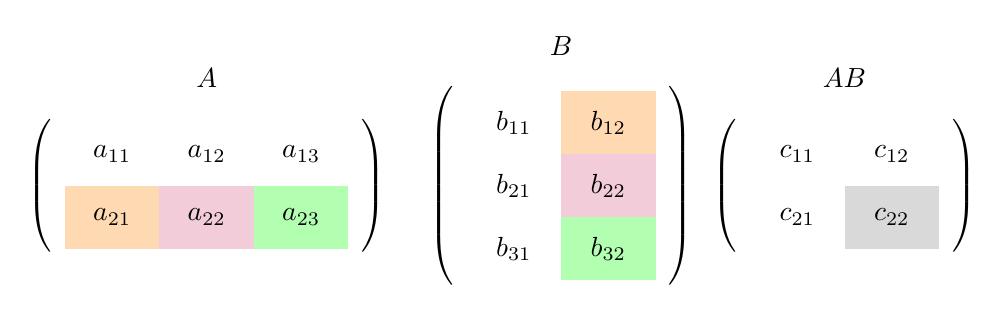
\begin{tikzpicture}[scale=0.9]
% Matrix A
\matrix (A) at (0,0) [matrix of math nodes, left delimiter=(, right delimiter=), nodes={minimum width=1.2cm, minimum height=0.8cm}] {
  a_{11} & a_{12} & a_{13} \\
  |[fill=orange!30]| a_{21} & |[fill=purple!20]| a_{22} & |[fill=green!30]| a_{23} \\
};
\node[above=0.2cm of A] {$A$};

% Matrix B
\matrix (B) at (5,0) [matrix of math nodes, left delimiter=(, right delimiter=), nodes={minimum width=1.2cm, minimum height=0.8cm}] {
  b_{11} & |[fill=orange!30]| b_{12} \\
  b_{21} & |[fill=purple!20]| b_{22} \\
  b_{31} & |[fill=green!30]| b_{32} \\
};
\node[above=0.2cm of B] {$B$};

% Result AB
\matrix (AB) at (9,0) [matrix of math nodes, left delimiter=(, right delimiter=), nodes={minimum width=1.2cm, minimum height=0.8cm}] {
  c_{11} & c_{12} \\
  c_{21} & |[fill=gray!30]| c_{22} \\
};
\node[above=0.2cm of AB] {$AB$};
\end{tikzpicture}
\end{center}

\vfill
Second diagonal entry:
$$c_{22} = \textcolor{orange!80!black}{a_{21}b_{12}} + \textcolor{purple!80!black}{a_{22}b_{22}} + \textcolor{green!50!black}{a_{23}b_{32}}$$
\end{frame}

\begin{frame}{Visual Proof: $\text{tr}(AB)$ — Combined}
Combining both diagonal entries:

\begin{align*}
\text{tr}(AB) &= c_{11} + c_{22} \\
&= (a_{11}b_{11} + a_{12}b_{21} + a_{13}b_{31}) \\
&\quad + (a_{21}b_{12} + a_{22}b_{22} + a_{23}b_{32})
\end{align*}

\vfill
This is the sum of all \x{color-matched pairs} from the two matrices.
\end{frame}

\begin{frame}[fragile]{Visual Proof: $\text{tr}(BA)$ — Same Colors!}
Now compute $BA$ (note: $B$ is $3 \times 2$, $A$ is $2 \times 3$, so $BA$ is $3 \times 3$):

\vfill
\begin{center}
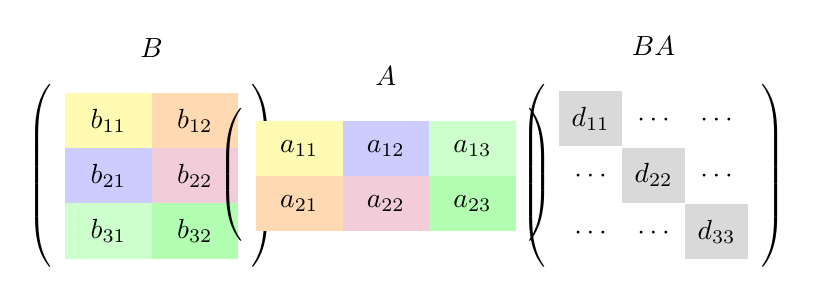
\begin{tikzpicture}[scale=0.85]
% Matrix B
\matrix (B) at (0,0) [matrix of math nodes, left delimiter=(, right delimiter=), nodes={minimum width=1.1cm, minimum height=0.7cm}] {
  |[fill=yellow!30]| b_{11} & |[fill=orange!30]| b_{12} \\
  |[fill=blue!20]| b_{21} & |[fill=purple!20]| b_{22} \\
  |[fill=green!20]| b_{31} & |[fill=green!30]| b_{32} \\
};
\node[above=0.2cm of B] {$B$};

% Matrix A
\matrix (A) at (3.5,0) [matrix of math nodes, left delimiter=(, right delimiter=), nodes={minimum width=1.1cm, minimum height=0.7cm}] {
  |[fill=yellow!30]| a_{11} & |[fill=blue!20]| a_{12} & |[fill=green!20]| a_{13} \\
  |[fill=orange!30]| a_{21} & |[fill=purple!20]| a_{22} & |[fill=green!30]| a_{23} \\
};
\node[above=0.2cm of A] {$A$};

% Result BA
\matrix (BA) at (7.5,0) [matrix of math nodes, left delimiter=(, right delimiter=), nodes={minimum width=0.8cm, minimum height=0.7cm}] {
  |[fill=gray!30]| d_{11} & \cdots & \cdots \\
  \cdots & |[fill=gray!30]| d_{22} & \cdots \\
  \cdots & \cdots & |[fill=gray!30]| d_{33} \\
};
\node[above=0.2cm of BA] {$BA$};
\end{tikzpicture}
\end{center}

\vfill
Diagonal entries of $BA$:
\begin{align*}
d_{11} &= b_{11}a_{11} + b_{12}a_{21} \\
d_{22} &= b_{21}a_{12} + b_{22}a_{22} \\
d_{33} &= b_{31}a_{13} + b_{32}a_{23}
\end{align*}
\end{frame}

\begin{frame}{Visual Proof: Conclusion}
$$\text{tr}(BA) = d_{11} + d_{22} + d_{33}$$

\begin{align*}
&= (b_{11}a_{11} + b_{12}a_{21}) + (b_{21}a_{12} + b_{22}a_{22}) + (b_{31}a_{13} + b_{32}a_{23})
\end{align*}

\vfill
By commutativity of multiplication ($a_{ij}b_{kl} = b_{kl}a_{ij}$):

\begin{align*}
&= (a_{11}b_{11} + a_{21}b_{12}) + (a_{12}b_{21} + a_{22}b_{22}) + (a_{13}b_{31} + a_{23}b_{32})
\end{align*}

\vfill
This is \x{exactly the same sum} as $\text{tr}(AB)$!

$$\boxed{\text{tr}(AB) = \text{tr}(BA)}$$

\x{Key}: The colored pairs are the same, just encountered in different order.
\end{frame}

\begin{frame}{Using Trace to Prove Dimension is Well-Defined}
\begin{thm}
If $V$ has two bases with $n$ and $m$ vectors respectively, then $n = m$.
\end{thm}

\vfill
\textbf{Proof strategy}:
\begin{enumerate}
\item Write one basis in terms of the other using change-of-basis matrices
\item Use left cancellation to show these matrices compose to identity
\item Use trace to count the sizes
\end{enumerate}
\end{frame}

\begin{frame}{Proof: Change of Basis Matrices}
Let $e_1, \ldots, e_n$ be one basis and $w_1, \ldots, w_m$ be another basis.

\vfill
Since $\{w_i\}$ is a basis, we can write each $e_j$ as a linear combination:
$$\begin{pmatrix} | & & | \\ e_1 & \cdots & e_n \\ | & & | \end{pmatrix} = \begin{pmatrix} | & & | \\ w_1 & \cdots & w_m \\ | & & | \end{pmatrix} P$$

for some $m \times n$ matrix $P$.

\vfill
Similarly, we can write:
$$\begin{pmatrix} | & & | \\ w_1 & \cdots & w_m \\ | & & | \end{pmatrix} = \begin{pmatrix} | & & | \\ e_1 & \cdots & e_n \\ | & & | \end{pmatrix} Q$$

for some $n \times m$ matrix $Q$.
\end{frame}

\begin{frame}{Proof: Composing the Changes}
Substituting the second equation into the first:

$$\begin{pmatrix} | & & | \\ e_1 & \cdots & e_n \\ | & & | \end{pmatrix} = \begin{pmatrix} | & & | \\ e_1 & \cdots & e_n \\ | & & | \end{pmatrix} QP$$

\vfill
Since $\{e_i\}$ are linearly independent, by \x{left cancellation}:
$$QP = I_n$$

\vfill
Similarly, substituting the first equation into the second:
$$\begin{pmatrix} | & & | \\ w_1 & \cdots & w_m \\ | & & | \end{pmatrix} = \begin{pmatrix} | & & | \\ w_1 & \cdots & w_m \\ | & & | \end{pmatrix} PQ$$

So $PQ = I_m$ by left cancellation.
\end{frame}

\begin{frame}{Proof: Using Trace}
We have:
\begin{itemize}
\item $QP = I_n$ (an $n \times n$ identity matrix)
\item $PQ = I_m$ (an $m \times m$ identity matrix)
\end{itemize}

\vfill
Taking traces:
$$\text{tr}(QP) = \text{tr}(I_n) = n$$
$$\text{tr}(PQ) = \text{tr}(I_m) = m$$

\vfill
But by the trace property $\text{tr}(QP) = \text{tr}(PQ)$:
$$n = m$$

\vfill
Therefore, \x{any two bases have the same number of vectors}! $\square$
\end{frame}

\begin{frame}{Definition: Dimension}
\begin{defi}[Dimension]
The \x{dimension} of a vector space $V$ is the number of vectors in any basis of $V$.

Notation: $\dim(V)$
\end{defi}

\vfill
This is \x{well-defined} because we just proved all bases have the same size!

\vfill
\x{Examples}:
\begin{itemize}
\item $\dim(\mathbb{R}^n) = n$ (basis: standard vectors $e_1, \ldots, e_n$)
\item $\dim(\text{Col}(A))$ = number of vectors in any basis for the column space
\end{itemize}
\end{frame}

% ═══════════════════════════════════════
% §5 RANK IS WELL-DEFINED
% ═══════════════════════════════════════
\section{Rank is Well-Defined}

\begin{frame}{Connecting Rank to Dimension}
\begin{thm}
The columns of $U$ from cross-filling $A = UV$ form a \x{basis} for $\text{Col}(A)$.
\end{thm}

\vfill
Therefore:
$$\text{rank}(A) = \text{number of columns of } U = \dim(\text{Col}(A))$$

\vfill
Since dimension is well-defined (doesn't depend on choice of basis), \x{rank is well-defined} (doesn't depend on pivot choices in cross-filling)!
\end{frame}

\begin{frame}{Why $U$ Forms a Basis — Preview}
The proof requires two parts:

\vfill
\textbf{Part 1}: Columns of $U$ \x{span} $\text{Col}(A)$

Every column of $A$ can be written as a linear combination of columns of $U$ (from $A = UV$).

\vfill
\textbf{Part 2}: Columns of $U$ are \x{linearly independent}

This comes from the triangular structure created by the pivot selection in cross-filling.

\vfill
(Full proof in next lecture — we need one more tool first)
\end{frame}

\begin{frame}{Summary}
\textbf{What we proved today}:

\begin{enumerate}
\item \x{Linear independence} = unique representation
\item \x{Left cancellation} property for independent columns
\item \x{Trace property}: $\text{tr}(AB) = \text{tr}(BA)$ (visual proof with colors)
\item \x{Dimension is well-defined}: All bases have the same size (using trace)
\item \x{Rank is well-defined}: rank$(A) = \dim(\text{Col}(A))$
\end{enumerate}

\vfill
\x{Big picture}: We elevated rank from an algorithmic definition to a \x{geometric property}.
\end{frame}

\end{document}
